In \autoref{abb:ProdukteRT} werden verwendbare Dienste von \ac{AWS}, gemeinsam mit ihren jeweiligen Einsatzgebieten gezeigt. In diesem Abschnitt soll besonders auf die Dienste zum Datenstreaming und zur Datenverarbeitung eingegangen werden. Gezeigt werden jedoch auch Dienste für -Speicherung, -Visualisierung und Machine Learning, da diese komplementär oder mit den prozessierten Daten verwendet werden können.
\begin{figure}[H]
\centering
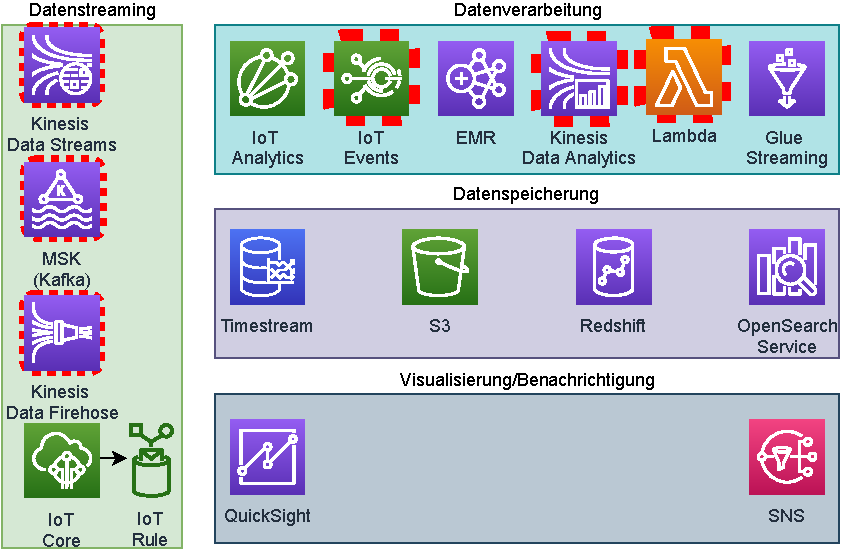
\includegraphics[width=\textwidth]{graphics/Overview-Realtime.pdf}
\caption{Einsetzbare Dienste im Bereich Echtzeitverarbeitung}
\label{abb:ProdukteRT}
\end{figure}

\TodoW{Hier noch besserer Übergang}

Innerhalb des \ac{IoT} Core Brokers ist es möglich, Regeln zu definieren, die einzelne Nachrichten aus Topics in andere Dienste weiterzuleiten. Dazu müssen besagte Nachrichten selektiert werden, was mittels eines SQL Dialekts möglich ist. Eine beispielhafte Selektion könnte folgendermaßen aussehen: \mintinline[breaklines]{sql}{SELECT * FROM 'iot-demo-sensor' WHERE device <> 'test'}
Alle Attribute jeder Nachricht, die Nicht vom Gerät test stammen, aus dem Topic iot-demo-sensor werden dabei selektiert und können dann z.B. weitergeleitet werden.

\subsection{AWS IoT Events}




Im Rahmen der \AWSIOT{} Familie von Diensten gibt es neben dem bereits angesprochenen \AWSIOT{} Analytics ebenfalls \AWSIOT{} Events.  
Der Dienst dient nach Angaben von Amazon der Konfiguration von \enquote{If-Then-Else} Regeln, mit denen Ereignisse (also Events) erkannt und verarbeitet werden sollen, indem Aktionen ausgelöst werden.\footcite[Vgl.][]{AmazonWebServicesInc..o.J.b} Die Abläufe können dabei, ähnlich wie bei Node-RED graphisch konfiguriert werden. Unterstützte Aktionen von \AWSIOT{} Events sind beispielsweise der Aufruf von Lambda oder Benachrichtigung via \ac{SNS}.\footcite[Vgl.][]{AmazonWebServicesInc..o.J.ao}
\begin{figure}[H]
\centering
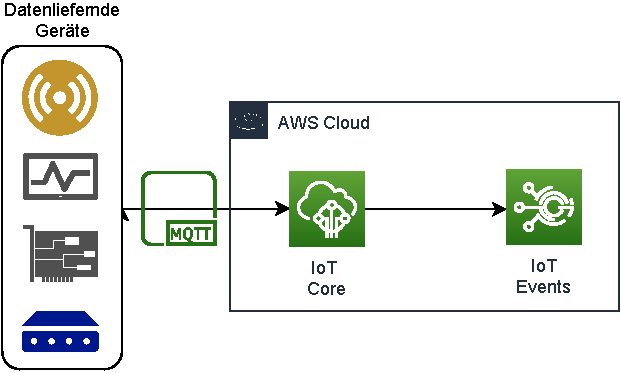
\includegraphics[width=0.8\textwidth]{graphics/IoT-Events-general.pdf}
\caption{Grobarchitektur des Ablaufes für IoT Events}
\label{abb:GrobArchitekturIoTEvents}
\end{figure}

\AWSIOT{} Events basiert auf abgebildeten Zuständen, die basierend auf ihren Übergängen Aktionen auslösen. \autoref{abb:BeispielIoTEvents} zeigt 3 beispielhaft 3 definierte Zustandsübergänge in der Weboberfläche von \AWSIOT{} Events. Jeder Kreis, welcher einen Zustand simbolisiert, hat 3 eigene Ereignisse, nämlich OnEnter, OnInput und OnExit. Zusätzlich sind Zustände mit Zustandsübergangspfeilen verbunden, welche basierend auf einer Ausführungskondition ausgelöst werden. Eine solche Ausführungskondition (auch Trigger genannt) wäre beispielsweise \mintinline[breaklines]{javascript}{$input.Input1.value > $variable.threshold}. Insgesamt funktioniert \AWSIOT{} Events also wie ein deterministischer Automat, da Zustandsübergänge genau definiert sind.
\begin{figure}[H]
\centering
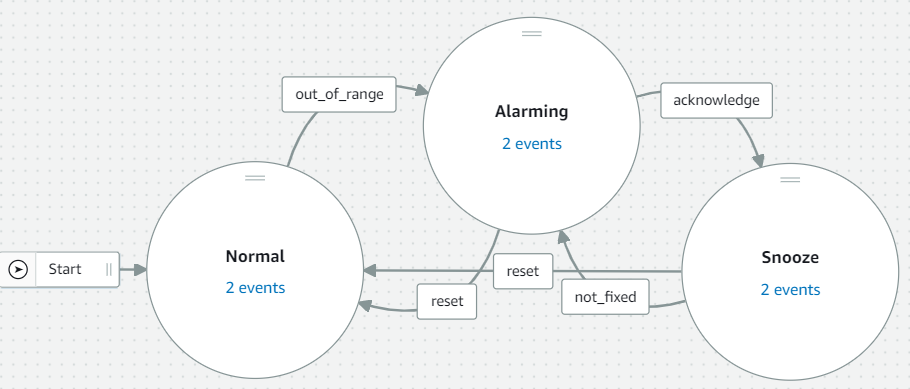
\includegraphics[width=\textwidth]{graphics/IoT-Events-Demo.png}
\caption{Beispiel IoT Events}
\label{abb:BeispielIoTEvents}
\end{figure}
Sollte ein Alarmzustand erreicht werden, können andere Dienste wie Lambda oder \ac{SNS} zur Verarbeitung oder Benachrichtigung integriert werden.

\subsubsection{Features des Dienstes}
\AWSIOT{} Events unterstützt reine \enquote{if-then-else} Überprüfungen. Trotzdem sind Variablen zur Evaluation selbstgeschriebener Logik verfügbar, womit sich zumindest ein Teil der gewünschten Features umsetzen lässt. Fakt ist dennoch, dass nur Analysen in einem endlichen zeitlichen Fenster durchführbar sind, welches durch Eingangsfrequenz und Anzahl der verwendeten Variablen beschränkt ist.\footcite[Vgl.][]{AmazonWebServicesInc..o.J.am} Eine Kalkulation eines Medians wäre (angenommen, dass die Werte sortiert gespeichert werden) wie folgt möglich, wenn 10 Variablen angenommen werden: \mintinline[breaklines]{javascript}{0.5*($variable.pastmeasure5 + $variable.pastmeasure6))}
Abseits von Schwellwertüberprüfungen, welche vorher definiert wurden, ist \AWSIOT{} Events nur mit großem Aufwand bei beschränkter Evaluationssprache zu weitergehenden Auswertungen fähig, welche immer von dem Zeitfenster, welches die Variablen abdecken abhängig ist. Ebenfalls sind keine selbstständigen Algorithmen zur Anomalieerkennung integriert.

\subsubsection{Performancegarantien}
\ac{AWS} gibt in der zu \AWSIOT{} Events zugehörigen \ac{SLA} keine Performancegarantien, sondern lediglich eine Verfügbarkeitsgarantie mit Penalen in Form von Rückzahlungen.\footcite[Vgl.][]{AmazonWebServicesInc..o.J.an} \AWSIOT{} Events hat dazu noch Limitierungen, wie beispielsweise das unveränderliche Limit von 10 Nachrichten pro Sekunde, die an einen Detektor gesendet werden können (also bei denen eigene Logik ausgeführt werden kann) oder das anpassbare Limit von 1000 Nachrichten, die pro Sekunde insgesamt evaluiert werden können.\footcite[Vgl.][]{AmazonWebServicesInc..o.J.ap}

\subsubsection{Gesamtkosten}
Im Folgenden werden für den Beispielusecase entsprechend der offiziellen Preisaufstellung von \ac{AWS} die monatlichen Nutzungskosten berechnet. \footcite[Vgl.][]{AmazonWebServicesInc..o.J.k}
\begin{table}[H]
\centering
\begin{tabular}{|l|l|l|}
\hline
Dimension & Preis(\$)/Einheit & Summe (\$) \\ \hline
evaluierte Regeln & \begin{tabular}[c]{@{}l@{}}0,000018/Regel\\ (teuerster Preis - ohne Volumenrabatt)\end{tabular} & 155,52 \\ \hline
Alarme & \begin{tabular}[c]{@{}l@{}}0,1/Alarm\\ (pro Sensor)\end{tabular} & 20 \\ \hline
\ac{SNS} (Push) & \begin{tabular}[c]{@{}l@{}}0,00002/Nachricht\\ (angenommen 5 Alarme/Gerät/Monat)\end{tabular} & 0,02 \\ \hline
% Lambda Ausführungen & \begin{tabular}[c]{@{}l@{}}0,0000002/Ausführung\\ 0,0000000167/GB-Sekunde\end{tabular} & 0,08 \\ \hline
% \begin{tabular}[c]{@{}l@{}}\ac{S3}-Speicher \\ (Lambda)\end{tabular} & 0,0245/GB Speicher & 0,0245 \\ \hline
Summe & \cellcolor[HTML]{EFEFEF} & \underline{175,6445} \\ \hline
\end{tabular}
\caption{Kostenvergleich AWS~IoT~Events}
\label{tab:kostenvergleich-AWS~IoT~Events}
\end{table}


\subsection{Amazon Kinesis}


Wenn über Kinesis gesprochen wird, ist zwischen mehreren Diensten zu differenzieren. Für diese Arbeit relevant sind Kinesis Data Streams, Kinesis Data Analytics und am Rande Kinesis Data Firehose, es gibt beispielsweise aber auch Kinesis Video Streams.

Mit Kinesis Data Streams ist der Dienst gemeint, der die Schnitstellen und Logik für das Streamen von Daten bereitstellt und Konsumenten wie Kinesis Data Analytics, \ac{EC2} oder Lambda unterstützt. 

Kinesis Data Analytics ist dafür ausgelegt, die Daten aus z.B. Kinesis Data Analytics nahe Echtzeit mittels \ac{SQL} Abfragen zu analysieren und z.B. Alarme auszulösen.

Kinesis Data Firehose dient dem Zweck, Daten aus z.B. Kinesis Data Analytics in Speichermedien/Datenbanken wie \ac{S3}, Redshift oder Elasticsearch Service zu übertragen.

Amazon Kinesis Data Analytics ist im Gegensatz zu \AWSIOT{} Analytics nicht allein auf die Analyse von \ac{IoT} Daten spezialisiert. Kinesis eignet sich vielmehr für generelle Analysen von allerlei Streamingdaten. Zusätzlich ist Amazon Kinesis (Data Streams) älter als \AWSIOT{} Analytics und bildet die technische Grundlage für die Verarbeitung \AWSIOT{} Events.\footcite[Vgl.][]{Pogosova.28.05.2020} Kinesis Data Streams wirbt damit, dass Daten in 70 Milisekunden nach Eingang zum Konsum verfügbar sind.\footcite[Vgl.][]{AmazonWebServicesInc..o.J.af}

Alternativ zur Kinesis Familie gibt es auch Open-Source Stream Analytics Dienste, wie von \citeauthor{Singh.2016} dargestellt.\footcite[Vgl.][]{Singh.2016} Diese kommen aufgrund der fehlenden Integration mit \ac{AWS} und des erhöhten Aufwands durch Eigenbetrieb nicht in Frage.

\begin{figure}[H]
\centering
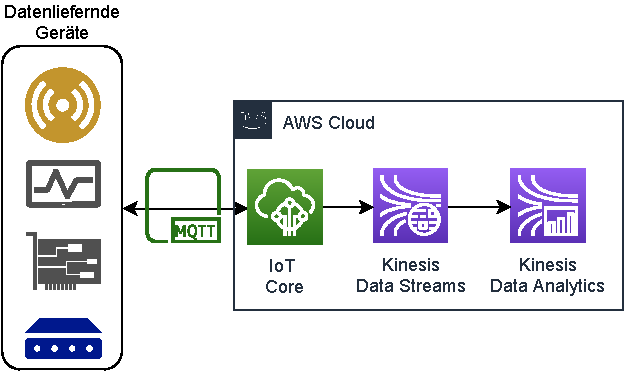
\includegraphics[width=0.8\textwidth]{graphics/Kinesis-Analytics-general.pdf}
\caption{Grobarchitektur des Ablaufes für Kinesis Analytics}
\label{abb:GrobArchitekturKinesisAnalytics}
\end{figure}
In \autoref{abb:GrobArchitekturKinesisAnalytics} ist das Zusammenspiel der Dienste aus der Kinesis Familie mit anderen Diensten dargestellt. Angenommen werden dabei die in \autoref{chap:rahmendatenverarbeitung} erläuterten Rahmenbedingungen, weshalb \ac{IoT} Core als Message Broker eingesetzt ist. Wie in der in \autoref{productselection:iotanalytics} beschriebenen Architektur, muss auch hier für die Datenverarbeitung eine Regel im \ac{IoT} Core Broker angelegt werden, um relevante Nachrichten an Kinesis Data Firehose weiterzuleiten.\footcite[Vgl.][]{AmazonWebServicesInc..o.J.} Die tatsächliche Analyse übernimmt der komplementäre Dienst Kinesis Data Analytics. 
In diesem Fall wurde angenommen, dass Kinesis Data Firehose die Datenübertragung vornimmt, da bei Kinesis Data Streams einzelne Shards, wie in \autoref{abb:KinesisShards} gezeigt, zu verwalten sind. Die Wahl von Kinesis Data Firehose bringt den NAchteil mit sich, dass die Daten nicht in Kinesis aufbewahrt werden können, was bei Data Streams möglich ist.\footcite[Vgl.][]{AmazonWebServicesInc..o.J.bh} Da die Daten aber in \ac{S3} von Kinesis Data Firehose persistiert werden und einzig das Volumen der durchgeleiteten Daten abgerechnet wird, ist die Verwendung von Firehose statt Streams unkomplizierter. Trotzdem kann, wenn benötigt Firehose mit Data Streams ersetzt werden, da beide mit Kinesis Data Analytics kompatibel sind.

\begin{figure}[H]
\centering
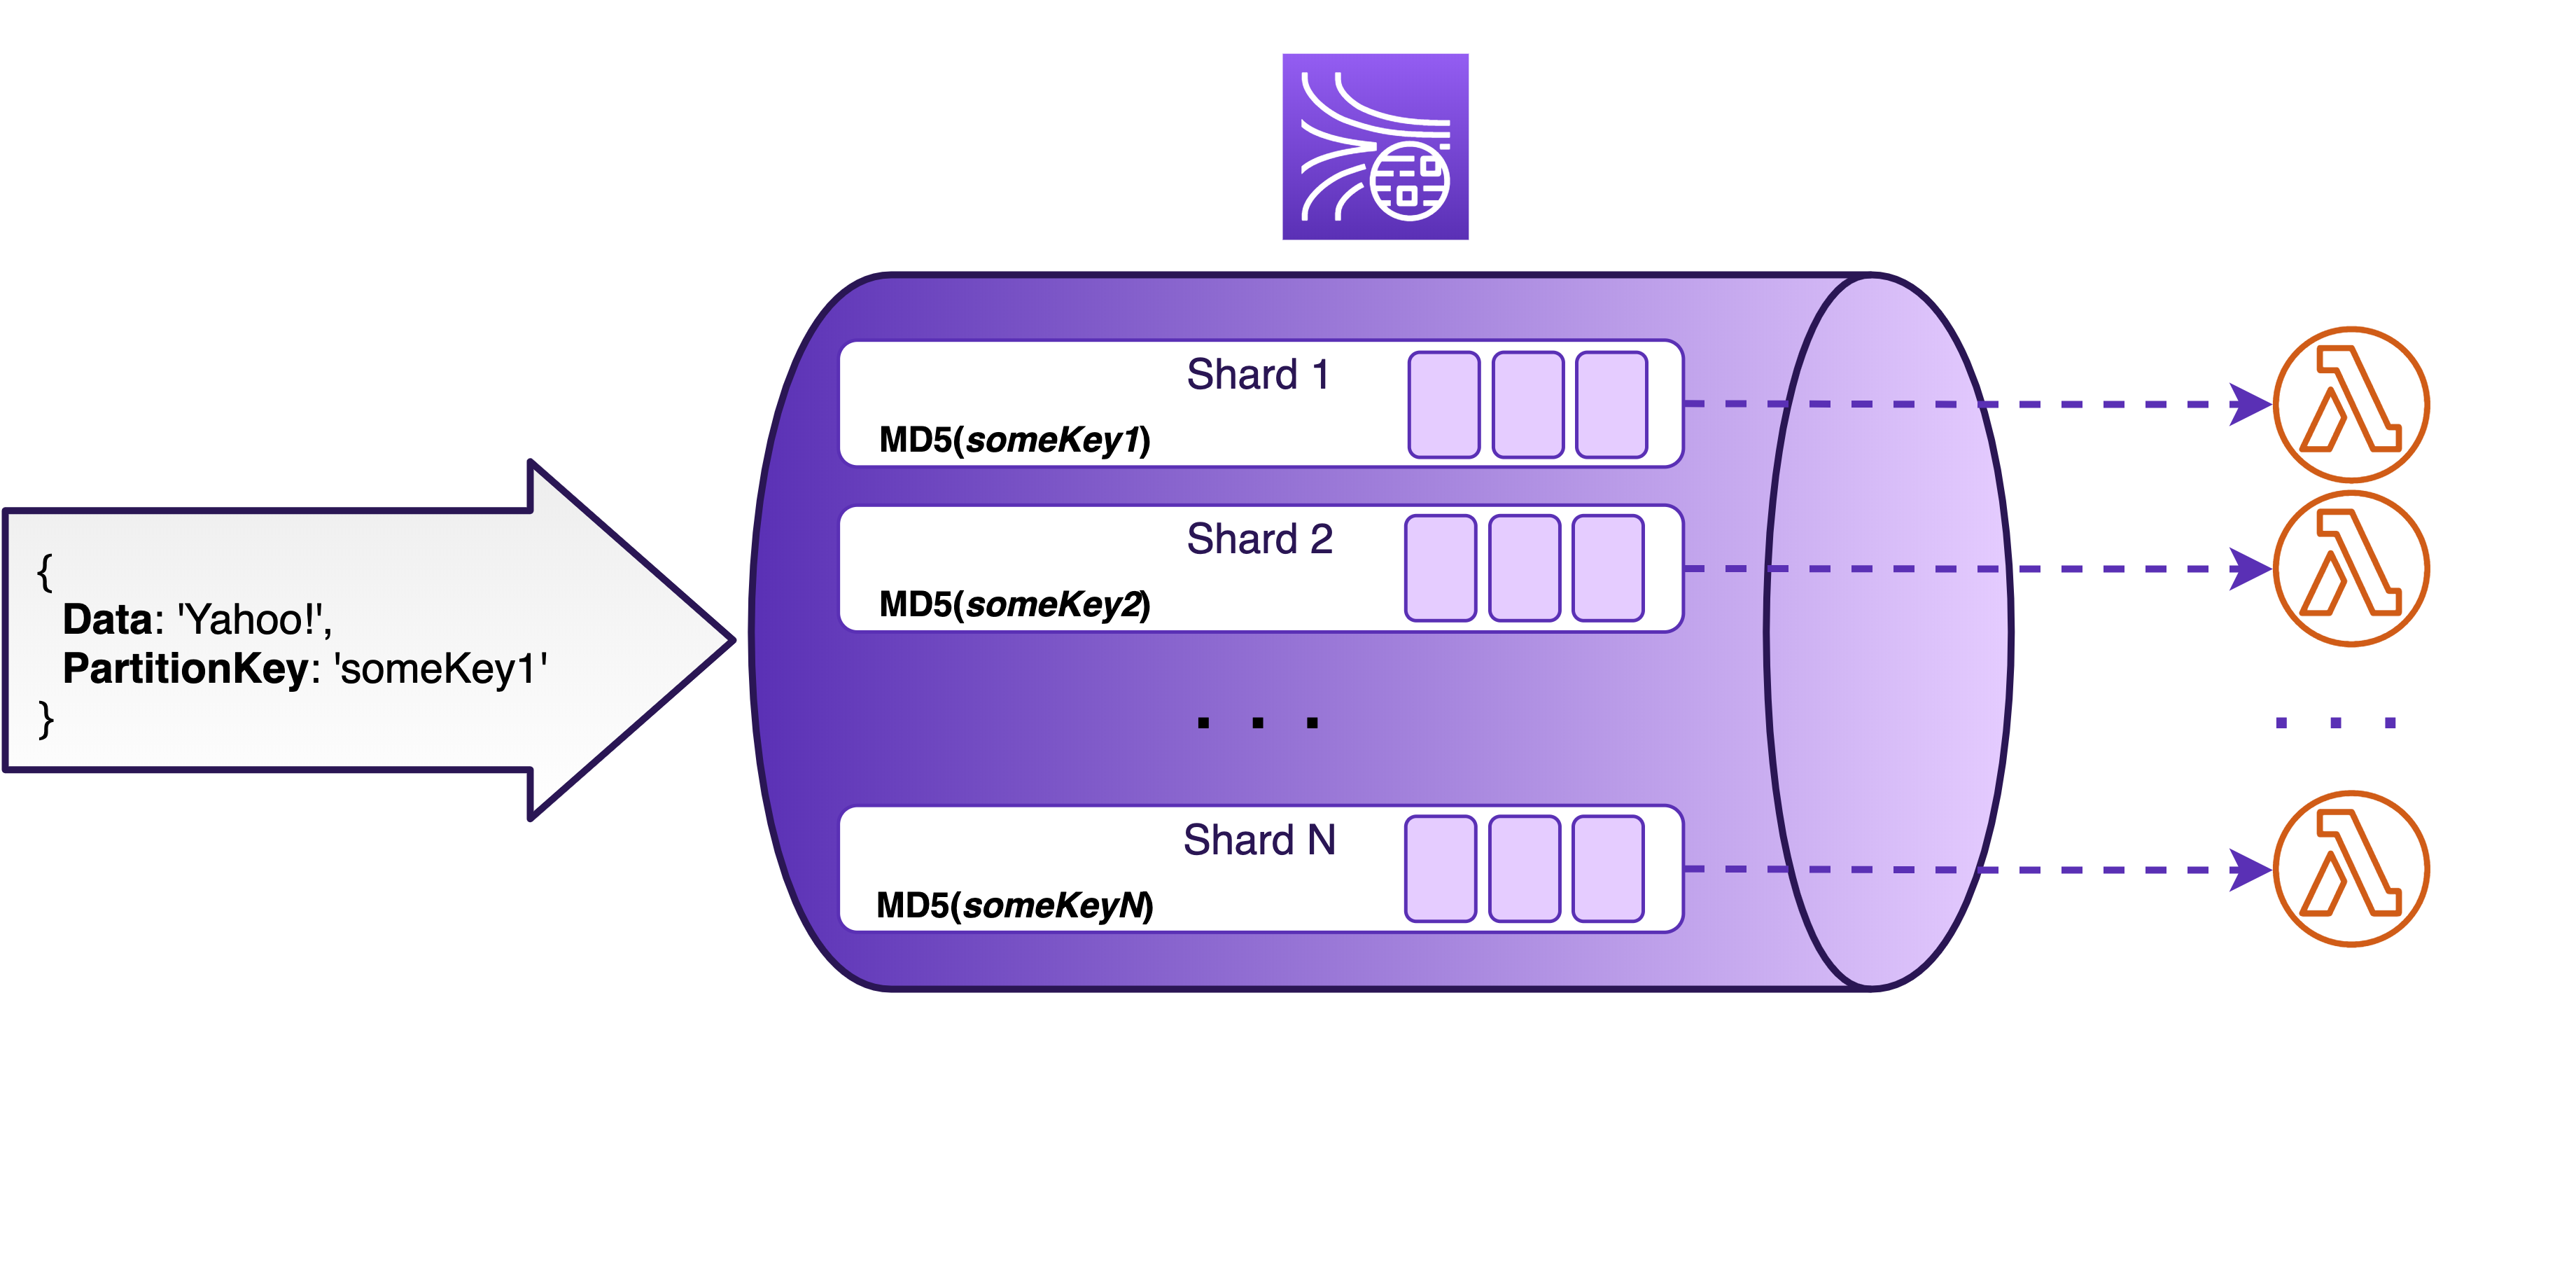
\includegraphics[width=\textwidth]{graphics/kinesis-inner-workings.png}
\caption[Funktionsweise von Kinesis]{Funktionsweise von Kinesis.\footnotemark}
\label{abb:KinesisShards}
\end{figure}
\footnotetext{Entnommen aus: \cite{Pogosova.28.05.2020}}

Kinesis Data Streams unterstützt, im Gegensatz zu Data Firehose, eine erweiterte Aufbewahrung $\lbrack$\textit{Data Retention}$\rbrack$, bei welcher Daten bis maximal 365 Tage nach initialem Einspielen erneut an Konsumenten wie Kinesis Data Analytics zur Verarbeitung gesendet werden können. Dies zieht Zusatzkosten nach sich. Treten jedoch Fehler in einer Analyse auf, kann diese für den gewählten Aufbewahrungszeitraum wiederholt werden.

Kinesis Data Analytics unterstützt sowohl die Datenanalyse mittels \ac{SQL} als auch mittels der programmatischen Schnittstellen, die das Open Source Projekt Apache Flink anbietet.\footcite[Vgl.][]{AmazonWebServicesInc..2020f} Der Analysecode, der die Schnittstellen von Flink verwendet, kann in Java, Scala oder Python geschrieben sein.

\subsubsection{Features des Dienstes}
Folgend werden die Funktionen der \ac{SQL}-Analyse von Kinesis Data Analytics dargestellt, da die Funktionalitäten der Flink-Schnittstelle abhängig sind von Programmiersprache und verwendeter Bibliotheken. 
Eine direkte Funktion um den Median oder Quantile zu berechnen, ist nicht vorhanden. \footcite[Vgl.][]{RyanN.2018} Statdessen ist aber eine Lösung mittels der \mintinline[breaklines]{sql}{group_rank} Funktion möglich, wie von \citeauthor{RyanN.2018} im \ac{AWS} Forum gezeigt.\footcite[Vgl.][]{AmazonWebServicesInc..o.J.as}\nzitat\footcite[Vgl.][]{RyanN.2018}
Mittels dem von \citeauthor{Guha.2016} gezeigten Random Cut Forest Algorithmus können Anomalien erkannt werden.\footcite[Vgl.][1]{Guha.2016} Dieser Algorithmus ist in Kinesis Data Analytics in Form der \\ \mintinline[breaklines]{sql}{RANDOM_CUT_FOREST_WITH_EXPLANATION} Funktion integriert.\footcite[Vgl.][]{AmazonWebServicesInc..o.J.ar}
Die Schwellwertüberschreitungserkennung ist mittels einer \ac{SQL} \mintinline{sql}{WHERE} Bedingung in der Abfrage machbar.
Der gleitende Durchschnitt lässt sich für Intervalle mittels der \mintinline[breaklines]{sql}{EXP_AVG} Funktion berechnen.\footcite[Vgl.][]{AmazonWebServicesInc..o.J.aq}
\citeauthor{Herman.2020} kritisiert bei Kinesis Data Analytics den angepassten \ac{SQL} Dialekt, welcher keine Interoperabilität zulässt und die fehlende Testbarkeit außerhalb von \ac{AWS} Werkzeugen.\footcite[Vgl.][]{Herman.2020}

\subsubsection{Performancegarantien}
Kinesis Data Streams bietet einen MB Durchsatz pro Sekunde und provisioniertem \enquote{Shard}. Da Kinesis Data Firehose auf Kinesis Data Streams aufbaut, ist ähnliches für Data Firehose anzunehmen\footcite[Vgl.][]{Pogosova.28.05.2020} 
% Mittels des \enquote{enhanced fanout} kann Kinesis gleichzeitig 2MB an Durchsatz pro Sekunde zu konsumierenden Applikationen bereitstellen.\footcite[Vgl. auch im Folgenden][]{Hunt.2018} 
\ac{AWS} bietet laut eigener Aussage mittels einer spezieller HTTP/2 \ac{API} auch eine Leseverzögerung von 70 Milisekunden, oder weniger.\footcite[Vgl.][]{AmazonWebServicesInc..o.J.af} 
Laut der \ac{AWS}-eigenen Dokumentation liegt die Ende zu Ende Verzögerung von Dateneinspeisung bis Konsumption typischerweise unter einer Sekunde. Dies weicht das eigentliche Marketingversprechen von 70 Milisekunden schon auf.\footcite[Vgl.][]{AmazonWebServicesInc..o.J.ae}
Die Kinesis \ac{SLA} enthält auch keine Klausel zur eigentlichen Performance, nur eine Garantie zur Verfügbarkeit von 99,99\% pro Monat.\footcite[Vgl.][]{AmazonWebServicesInc..o.J.ad} 
% Es ist Abwägungssache, ob der Subsekunden Latenz von Kinesis Data Streams Glauben geschenkt wird, beziehungsweise ob die Latenz im Subsekunden Bereich überhaupt relevant ist, oder ob alles kleiner fünf Sekunden als nahe genug an der Echtzeit akzeptiert wird.

Es gab bis jetzt ein schweres Ereignis, bei dem Kinesis in einer Region für den Zeitraum von 12 Stunden beeinträchtigt war und andere, von Kinesis abhängige Dienste beeinträchtigte.\footcite[Vgl. auch im Folgenden][]{AmazonWebServicesInc..2020e} Dieses Ereignis war jedoch auf die \enquote{us-east-1} Region begrenzt und die Auswirkungen konnten durch Migration auf andere Regionen, wie beispielsweise \enquote{eu-central-1} für Nutzende mitigiert werden.

\subsubsection{Gesamtkosten}
Für die Gesamtschätzung wurde Kinesis Data Firehose mit Streaming zu \ac{S3} und Kinesis Data Analytics angesetzt.\footcite[Vgl. auch im Folgenden][]{AmazonWebServicesInc..o.J.bi} Zusätzlich wurde angenommen, dass Analysen mittels \ac{SQL} erfolgen, da wie gezeigt genügend der erwünschten Features vorhanden sind. Kinesis Data Firehose rundet Datensätze auf die nächsten 5KB auf.
\begin{table}[H]
\centering
\begin{tabular}{|l|l|l|}
\hline
Dimension & Preis(\$)/Einheit & Summe (\$) \\ \hline
Kinesis Data Firehose & 0,033/GB & 1,38 \\ \hline
\ac{S3}-Speicher & 0,0245/GB Speicher & 0,64 \\ \hline
\begin{tabular}[c]{@{}l@{}}Kinesis Data Analytics\\ Processing Unit\end{tabular} & 0,132/h & 32,12 \\ \hline
\ac{SNS} (Push) & \begin{tabular}[c]{@{}l@{}}0,00002/Nachricht\\ (angenommen 5 Alarme/Gerät/Monat)\end{tabular} & \textless{}0,02 \\ \hline
Lambda Ausführungen & \begin{tabular}[c]{@{}l@{}}0,0000002/Ausführung\\ 0,0000166667/Sekunde (angenommen: 5)\\ 0,0000000167/GB \acs{RAM}/ms\end{tabular} & 0,08 \\ \hline
Summe & \cellcolor[HTML]{EFEFEF} & \underline{34,24} \\ \hline
\end{tabular}
\caption{Kostenvergleich Amazon~Kinesis}
\label{tab:kostenvergleich-Amazon~Kinesis}
\end{table}
 Zusätzlich wird angenommen, das \ac{SQL}-Statements ausgeführt werden, welche als \enquote{Processing units} abgerechnet werden.\footcite[Vgl. auch im Folgenden][]{AmazonWebServicesInc..o.J.m} Da Kinesis Data Analytics nicht selbstständig mit \ac{SNS} kommunizieren kann, wird Lambda als Weiterleitungsplattform für Alarme mit angesetzt.\footcite[Vgl.][]{AmazonWebServicesInc..2017b} 

Preise für Kinesis Data Streams wären die Folgenden, unter der Annahme, dass \ac{S3} wegfällt, da Kinesis Data Streams die Daten selber zwischenspeichern kann:\footcite[Vgl. auch im Folgenden][]{AmazonWebServicesInc..o.J.l}
\begin{table}[H]
\centering
\begin{tabular}{|l|l|l|}
\hline
Dimension & Preis(\$)/Einheit & Summe (\$) \\ \hline
\begin{tabular}[c]{@{}l@{}}Kinesis Data Streams\\ Shard-Stunde\end{tabular} & 0,018/h & 13,14 \\ \hline
\begin{tabular}[c]{@{}l@{}}Kinesis Data Streams\\ PUT-Operationen\end{tabular} & 0,0175/Million & 0,15 \\ \hline
\begin{tabular}[c]{@{}l@{}}Kinesis Data Analytics\\ Processing Unit\end{tabular} & 0,132/h & 32,12 \\ \hline
\ac{SNS} (Push) & \begin{tabular}[c]{@{}l@{}}0,00002/Nachricht\\ (angenommen 5 Alarme/Gerät/Monat)\end{tabular} & \textless{}0,02 \\ \hline
Lambda Ausführungen & \begin{tabular}[c]{@{}l@{}}0,0000002/Ausführung\\ 0,0000166667/Sekunde (angenommen: 5)\\ 0,0000000167/GB \acs{RAM}/ms\end{tabular} & 0,08 \\ \hline
Summe & \cellcolor[HTML]{EFEFEF} & \underline{45,51} \\ \hline
\end{tabular}
\caption{Kostenvergleich Amazon~Kinesis~Data~Streams}
\label{tab:kostenvergleich-Amazon~Kinesis~Data~Streams}
\end{table}




\subsection{AWS Lambda}\label{chap:vergleich-lambda}


Bei \ac{AWS} Lambda handelt es sich um die Amazon Implementierung eines \ac{FaaS} Dienstes. Innerhalb dieser Arbeit wird Lambda als einzige generelle Computing Plattform betrachtet, da Alternativen wie \ac{EC2}, welches virtuelle Maschinen anbietet oder \ac{ECS}, welches Container anbietet einen von einzelnen Events unabhängigen Lebenszyklus haben. 
So laufen Container auf \ac{ECS} oder virtuelle Maschinen auf \ac{EC2}, wenn nicht anders konfiguriert kontinuierlich und holen/ \enquote{fetchen} Daten. In Zeiträumen, in denen keine Daten bereitstehen, sind die entsprechenden Container und virtuellen Maschinen im Leerlauf, was unnötige Kosten erzeugt. Lambda hingegen wird von unterstützenden Diensten zur Verarbeitung von Events aufgerufen. 
Dabei ist je nach Dienst einstellbar, ob ein Aufruf pro Event stattfinden soll, oder Events zu einer konfigurierbaren Anzahl gruppiert werden und dann an Lambda übergeben werden. Lambda eignet sich besonders für analytische Workloads, seit der kürzlichen Addition von Intels \ac{AVX2}.\footcite[Vgl. auch im Folgenden][]{Beswick.24.11.2020} \ac{AVX2} ist ein spezieller CPU-Instruktionssatz, der die Verarbeitung von Vektorinstruktionen beschleunigt. Diese kommen besonders häufig in der Statistik oder bei dem Machine Learning vor. 
Aufgrund der zentralen Rolle im Bereich Compute bei \ac{AWS}, können viele Dienste Events an Lambda senden. In \autoref{abb:GrobArchitekturLambda} sind als Integrationsbeispiele die \acp{MoM} \ac{IoT} Core, MQ und Kinesis Data Streams als Eventlieferanten gezeigt.
\begin{figure}[H]
\centering
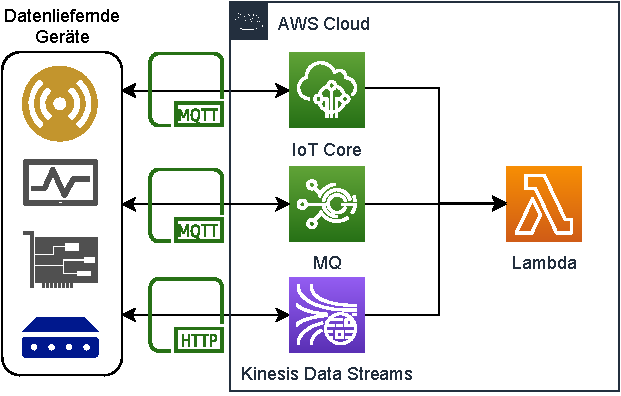
\includegraphics[width=0.8\textwidth]{graphics/Lambda-general.pdf}
\caption{Grobarchitektur des Ablaufes für Lambda}
\label{abb:GrobArchitekturLambda}
\end{figure}

\subsubsection{Features des Dienstes}
Da Lambda eine programmierbare Plattform ist, welche mehrere Sprachen unterstützt, muss im Folgenden eine Programmiersprache angenommen werden. Python hat in einer Umfrage von Kaggle unter Datenwissenschaftlern die höchste Popularität, gefolgt von \ac{SQL} ausgemacht. Aus diesem Grund wird im Folgenden von der Verwendung der Programmiersprache Python ausgegangen (speziell auch, da sich eine Umsetzung mit \ac{SQL} in Lambda schwierig gestalten würde).\footcite[Vgl.][]{Hayes.2020} Gemäß einer Analyse des Entwicklerportals Stack Overflow ist das Paket \enquote{pandas} dabei die populärste Programmbibliothek für Datenwissenschaft.\footcite[Vgl.][]{Robinson.2017} Aus diesem Grund wird im Folgenden die Verwendung von Python mit pandas in Lambda angenommen. Angenommen wird, dass das an Lambda übermittelte Bearbeitungsfenster groß genug war, um Analysen zuzulassen.
\newcommand{\pandasmethod}[1]{\mintinline[breaklines]{python}{pandas.#1()}}
In pandas können Quantile mittels der \pandasmethod{DataFrame.quantile} Methode berechnet werden.\footcite[Vgl.][]{o.V..o.J.c} Für den Median ist eine eigene Methode verfügbar, \pandasmethod{DataFrame.median}. \footcite[Vgl.][]{o.V..o.J.d}
\citeauthor{Bartos.2019} haben den Random Cut Forest Algorithmus von \citeauthor{Guha.2016} in Python zur Verwendung mit pandas als seperate Bibliothek implementiert und OpenSource bereitgestellt.\footnote{Siehe: \url{https://github.com/kLabUM/rrcf}}\nzitat\footcite[Vgl.][]{Bartos.2019} Es gibt, wie bei den anderen Diensten gezeigt, viele weitere Methoden zur Anomalieerekennung, welche programmatisch implementiert werden könnten.
Schwellwertüberschreitungen können mittels \pandasmethod{DataFrame.gt} überprüft werden, wobei \enquote{gt} für \enquote{greater-than} steht.\footcite[Vgl.][]{o.V..o.J.e}
Ein exponentieller gleitender Durchschnitt lässt sich, wie von \citeauthor{Sharma.2019} gezeigt, mittels der folgenden, verketteten, Methoden berechnen: \pandasmethod{DataFrame.ewm().mean}.\footcite[Vgl.][]{Sharma.2019} 

\subsubsection{Performancegarantien}
\ac{AWS} bietet für Lambda in dem \ac{SLA} eine 99,\textbf{95} \% garantierte Verfügbarkeit an.\footcite[Vgl.][]{AmazonWebServicesInc..2019d}

Die Zuweisung von \ac{RAM} und daran gekoppelt vCPUs erfolgt bei Lambda dynamisch und ist vom Nutzer einzustellen. Um dies für Nutzende einfacher zu machen, gibt es das Projekt Lambda Power Tuning, welches die optimale \ac{RAM}-/Leistungskonfiguration für Funktionen ermittelt durch mehrere Tests.\footcite[Vgl. auch im Folgenden][]{AmazonWebServicesInc..o.J.at} Da höhere \ac{RAM} Einstellungen mehr kosten, kann für optimale Leistung oder für das Preis/Leistungsoptimum optimiert werden.

Wie von \citeauthor{Madden.2019} gezeigt, eignet sich Lambda für die Verarbeitung großer Datensätze. 
Dies wurde mit der Verarbeitung von 259 TB Daten in knapp 20 Minuten demonstriert.\footcite[Vgl. auch im Folgenden][]{Madden.2019} Speziell heben \citeauthor{Madden.2019} auch hervor, dass Lambda von keiner Last zu knapp zwei Millionen Einträgen pro Sekunde und zurück skaliert hat.

\subsubsection{Gesamtkosten}
\autoref{tab:kostenvergleich-AWS~Lambda~Maximal} zeigt die möglichen Kosten, wenn für jede eingehende Nachricht eine Lambdafunktion aufgerufen und ausgeführt wird (unabhängig davon, dass das mit den Standardeinstellungen für Parallelität nicht realisierbar wäre).
\begin{table}[H]
\centering
\begin{tabular}{|l|l|l|}
\hline
Dimension & Preis(\$)/Einheit & Summe (\$) \\ \hline
Lambda Ausführungen & 0,0000002/Ausführung & 1,728 \\ \hline
Lambda \ac{RAM} & 0,0000000167/GB-Sekunde & 720 \\ \hline
\ac{S3}-Speicher & 0,0245/GB Speicher & 0,0006 \\ \hline
\ac{SNS} (Push) & \begin{tabular}[c]{@{}l@{}}0,00002/Nachricht\\ (angenommen 5 Alarme/Gerät/Monat)\end{tabular} & 0,02 \\ \hline
Summe & \cellcolor[HTML]{EFEFEF} & \underline{721,75} \\ \hline
\end{tabular}
\caption{Kostenvergleich AWS~Lambda~Maximal}
\label{tab:kostenvergleich-AWS~Lambda~Maximal}
\end{table}

Um diese hohen Kosten zu mitigieren, gibt es mehrere Varianten. Folgend wird auf die Zwischenschaltung einer \ac{MoM}, nämlich \ac{AWS} \ac{SQS} und auf die Vorfilterung der Nachrichten durch \AWSIOT{} Core Rules näher eingegangen.

\autoref{abb:Lambda-Batch} zeigt die Zwischenschaltung von \ac{SQS} als Puffer, von dem asynchron gelesen werden kann.

\begin{figure}[H]
\centering
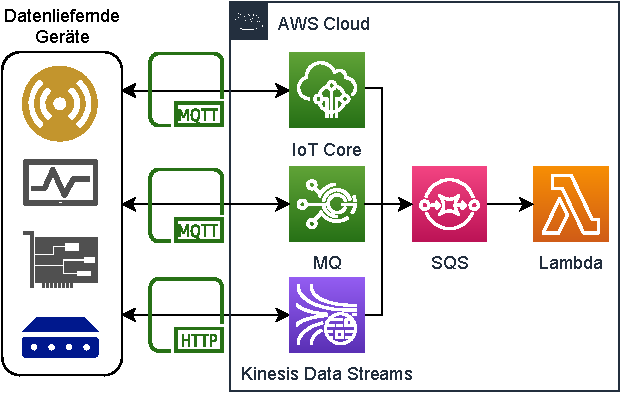
\includegraphics[width=0.8\textwidth]{graphics/Lambda-Batch.pdf}
\caption{Lambda Sammelverarbeitung via SQS}
\label{abb:Lambda-Batch}
\end{figure}

Seit November 2020 ist es in Lambda möglich, mittels der Einstellung \enquote{MaximumBatchingWindowInSeconds} das Übertragungsfenster frei zu definieren, in welchem auf Nachrichten von \ac{SQS} gewartet wird.\footcite[Vgl. auch im Folgenden][]{AmazonWebServicesInc..2020b} Dies erlaubt innerhalb eines maximalen Fensters von fünf Minuten Nachrichten zu sammeln und an Lambda zu übermitteln. Dies reduziert entsprechend die Ausführungen auf 20 pro Stunde und ist, wie in \autoref{tab:kostenvergleich-AWS~Lambda~Sammelverarbeitung} zu sehen, wesentlich günstiger.

\begin{table}[H]
\centering
\begin{tabular}{|l|l|l|}
\hline
Dimension & Preis(\$)/Einheit & Summe (\$) \\ \hline
Lambda Ausführungen & 0,0000002/Ausführung & 0,0029 \\ \hline
Lambda \ac{RAM} & 0,0000000167/GB-Sekunde & 1,2 \\ \hline
\ac{S3}-Speicher & 0,0245/GB Speicher & 0,0006 \\ \hline
\ac{SQS}-Durchsatz & 0,40/Million Anfragen & 3,456 \\\hline
\ac{SNS} (Push) & \begin{tabular}[c]{@{}l@{}}0,00002/Nachricht\\ (angenommen 5 Alarme/Gerät/Monat)\end{tabular} & 0,02 \\ \hline
Summe & \cellcolor[HTML]{EFEFEF} & \underline{4,6795} \\ \hline
\end{tabular}
\caption{Kostenvergleich AWS~Lambda~Sammelverarbeitung}
\label{tab:kostenvergleich-AWS~Lambda~Sammelverarbeitung}
\end{table}


Alternativ ist mittels einer angepassten Regel in \AWSIOT{} Rules, die in \autoref{listing:iot-rule-threshold} gezeigt ist, eine Ausführung nur bei Überschreitung des Schwellwerts möglich.

\begin{listing}[H]
\inputminted[frame=lines,breaklines=true]{sql}{code/iot-rules-lambda-filter.sql}
\caption{IoT Rule Schwellwertregel}
\label{listing:iot-rule-threshold}
\end{listing}
Diese Regel reduziert die rechnerischen Ausführungen auf 1000 pro Monat. Wie in \autoref{tab:kostenvergleich-AWS~Lambda~IOT~Sammelverarbeitung} gezeigt, fallen die Kosten bei 1000 Ausführung noch geringer als bei der gepufferten Variante mit \ac{SQS} aus. Es ist abhängig, ob eine Schwellwertüberprüfung in \AWSIOT{} Rules, speziell unter dem Paradigma der \enquote{Immutable Infrastructure}, welche unveränderliche, versionsverwaltete Infrastruktur fordert, als akzeptabel angesehen wird.\footcite[Vgl.][]{AmazonWebServicesInc..o.J.p} Für Änderungen an Schwellwerten müsste nämlich entsprechend die \AWSIOT{} Rule angepasst werden, was im \ac{SQS} durch eine einfach einzuspielende Codeänderung machbar wäre.

\begin{table}[H]
\centering
\begin{tabular}{|l|l|l|}
\hline
Dimension & Preis(\$)/Einheit & Summe (\$) \\ \hline
Lambda Ausführungen & 0,0000002/Ausführung & 0,0002 \\ \hline
Lambda \ac{RAM} & 0,0000000167/GB-Sekunde & 0,0833 \\ \hline
\ac{S3}-Speicher & 0,0245/GB Speicher & 0,0006 \\ \hline
\ac{SNS} (Push) & \begin{tabular}[c]{@{}l@{}}0,00002/Nachricht\\ (angenommen 5 Alarme/Gerät/Monat)\end{tabular} & 0,02 \\ \hline
Summe & \cellcolor[HTML]{EFEFEF} & \underline{0,1041} \\ \hline
\end{tabular}
\caption{Kostenvergleich AWS~Lambda~IOT~Sammelverarbeitung}
\label{tab:kostenvergleich-AWS~Lambda~IOT~Sammelverarbeitung}
\end{table}


\subsection{Amazon MSK / ksqlDB}


Bei \ac{MSK} handelt es sich um einen Managed Service für die Open Source Lösung Apache Kafka. Im Gegensatz zu anderen, hier im Kapitel aufgeführten Lösungen wie \ac{IoT} Analytics, hat Amazon \ac{MSK} nicht von Grund auf selber entwickelt, sondern einen großen Teil des Codes von Apache Kafka übernommen. Dies erklärt auch, warum die Anbindung an andere Dienste von Amazon bedeutend schwieriger ist, als beispielsweise an \ac{IoT} Core. In der in \autoref{abb:GrobArchitekturMSK} abgebildeten Grobarchitektur müsste zur Anbindung von Apache Kafka an zuliefernde Geräte ein Intermediär wie \ac{IoT} Core verrwendet werden, da Apache Kafka ein eigenes, binäres Protokoll hat, welches sonst in die Geräte implementiert werden müsste. \TodoW{letzten Halbsatz belegen} Fraglich ist, ob sich eine Implementierung des Kafka Protokolls auf allen Endgeräten lohnt, speziell im Licht besser unterstützter Standards wie \ac{MQTT}. Umgangen werden kann die Implementierung des Kafka Protokolls auf zuliefernden Geräten auf dreierlei Arten: Zum einen lassen sich mittels Kafka Connect for \ac{MQTT} \ac{MQTT} Broker als Eventquellen anbinden.\footcite[Vgl.][]{Erber.12.01.2021} Alternativ kann Kafka auch als \ac{MQTT} Proxy dienen, was bedeutet, dass Kafka als eigenständiger MQTT Broker agiert, wobei zu beachten ist, dass Kafka weit nicht alle \ac{MQTT} Standardelemente implementiert und eine paralelle Weiterverarbeitung in anderen Amazon Diensten nicht möglich ist.\footcite[Vgl.][]{Erber.12.01.2021} Zuletzt gibt es noch die Möglichkeiten, die Nachrichten via \ac{IoT} Core innerhalb von \ac{AWS} an \ac{MSK} weiterzuleiten, was auch in \autoref{abb:GrobArchitekturMSK} dargestellt ist.
\begin{figure}[H]
\centering
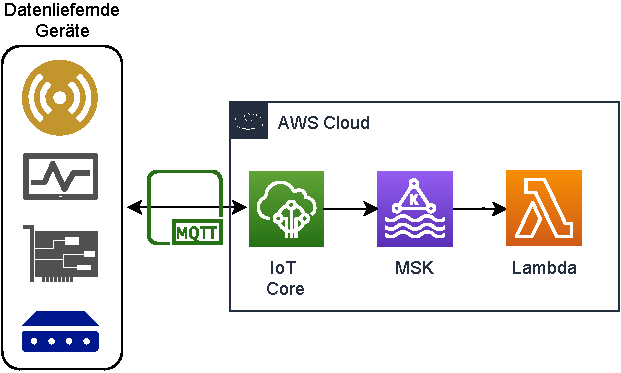
\includegraphics[width=0.8\textwidth]{graphics/MSK-general.pdf}
\caption{Grobarchitektur des Ablaufes für Managed Streaming for Apache Kafka}
\label{abb:GrobArchitekturMSK}
\end{figure}

Kafka selber fungiert nur als Broker für Daten. Da sich aber im Laufe der Zeit im Kafka Ökosystem Angebote wie ksqlDB entwickelt haben, welche nur mit Kafka funktionieren werden diese betrachtet. Möglich, aber kostenintensiv (durch Weiterleitung \ac{IoT} Core  $\rightarrow$ MSK  $\rightarrow$ Lambda) wäre die Weiterleitung auch an Lambda. Stattdessen soll aber ksqlDB die Verarbeitung übernehmen. Dieses wird wie sein Vorgänger KSQL hautpsächlich von der Firma Confluent, Inc. als OpenSource entwickelt und dient der Verarbeitung von Kafka Daten mittels \ac{SQL} in Form einer Streamverarbeitung.\footcite[Vgl.][]{Kreps.2019}\nzitat\footcite[Vgl.][]{Narkhede.2017} KSQL/ksqlDB kann wie von \citeauthor{Penz.2020} gezeigt, in \ac{AWS} in einem Container in \ac{ECS} oder in einer virtuellen Maschine, in \ac{EC2} betrieben werden.


\subsubsection{Features des Dienstes}
Im Folgenden wird der Featureumfang von ksqlDB näher beleuchtet.
Die Berechnung eines Medians/von Perzentilen scheint in ksqlDB nicht trivial machbar zu sein.
Wie von \citeauthor{Waehner.2018} gezeigt, ist es möglich in den ksql eigenen \acp{UDF}, in welchen eigener Code ausgeführt wird, Anomalieerkennung basierend auf Machine Learning durchzuführen.\footcite[Vgl.][]{Waehner.2018}
Eine Schwellwertüberschreitung kann mittels einer \mintinline[breaklines]{sql}{WHERE} Bedingung festgestellt werden.
Ein gleitender Durchschnitt kann ebenfalls mittels einer \ac{UDF} realisiert werden.\footcite[Vgl.][]{ConfluentInc..o.J.c} 
Diese berechnet den gleitenden Durchschnitt mit eigenem Code.

\subsubsection{Performancegarantien}
Da die Ressourcen für ksqlDB selbst eingestellt werden können, ist eine absolute Performanceaussage nicht möglich. Zusätzlich müssen zugehörige Ressourcen entweder selbst verwaltet werden oder als managed service von Confluent bezogen werden.
Die \ac{SLA} von \ac{MSK} definiert als Verfügbarkeitsziel 99,9\%, jedoch keine weiteren Performanceziele.\footcite[Vgl.][]{AmazonWebServicesInc..2019e} 
Die Performance von \ac{MSK} ist aufgrund des unterliegenden Instanzmodells wesentlich durch die Nutzenden beeinflussbar und ggf. durch vertikale Skalierung verbesserbar.
In einem Performancetest, den \ac{AWS} für \citeauthor{Statz.2019} durchgeführt hat, wurde als machbare Eingangsrate 310MB/Sekunde bei 15 provisionierten Brokern für möglich erklärt.\footcite[Vgl.][]{Statz.2019} 

\subsubsection{Gesamtkosten}
Wie von \citeauthor{Beswick.2020} dargestellt und in \autoref{abb:NetworkingMSK} gezeigt, muss MSK in mindestens zwei Availability Zones gestartet werden.\footcite[Vgl. auch im Folgenden][]{Beswick.2020} Dabei ist es für weniger kritische Systeme, wie hier gezeigt möglich, nur ein \ac{NAT}-Gateway zu verwenden, welches Konnektivität zum Internet ermöglicht (ohne eingehenden Traffic zu erlauben). Für kritische Lasten sollte ksqldb und das \ac{NAT}-Gateway in das zweite Subnetz repliziert werden.
\begin{figure}[H]
\centering
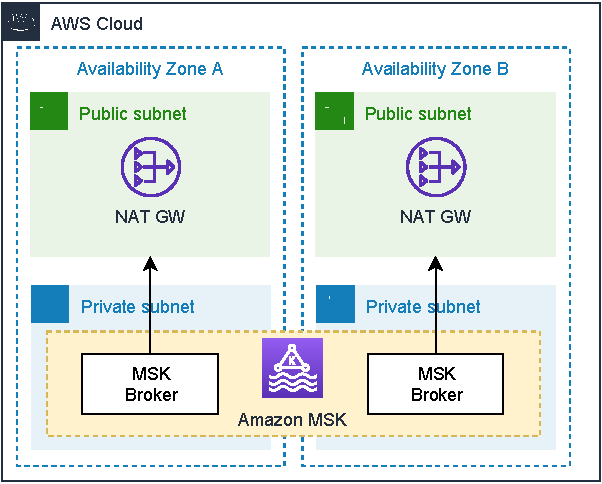
\includegraphics[width=0.55\textwidth]{graphics/MSK-Networking.pdf}
\caption{Networking MSK}
\label{abb:NetworkingMSK}
\end{figure}

Um ksqlDB zu betreiben, wird im folgenden angenommen, dass ein \acf{ECS} Container mit 1vCPU, 4GB \ac{RAM} und 10GB \ac{EFS} Speicherplatz provisioniert werden muss. Zusätzlich werden zwei \ac{MSK}-Brokerinstanzen, welche auf unterliegenden \ac{EC2}-Servern basieren, provisioniert.\footcite[Vgl.][]{AmazonWebServicesInc..o.J.o} Zusätzlich wurde ein \ac{NAT}-Gateway (für Updates und ausgehenden Traffic) mit 2GB Datendurchsatz angesetzt. Der Kostenvergleich ist in \autoref{tab:kostenvergleich-Amazon~MSK} gezeigt.

\begin{table}[H]
\centering
\begin{tabular}{|l|l|l|}
\hline
Dimension & Preis(\$)/Einheit & Summe (\$) \\ \hline
\begin{tabular}[c]{@{}l@{}}Broker Instanz\\ (t3.small - 2 mal)\end{tabular} & 0,0526/h & 76,7960 \\ \hline
Broker Storage & 0,119/h & 0,714 \\ \hline
\begin{tabular}[c]{@{}l@{}}\ac{NAT} Gateway\\ Zeit\end{tabular} & 0,052/h & 37,96 \\ \hline
\begin{tabular}[c]{@{}l@{}}\ac{NAT} Gateway\\ Durchsatz\end{tabular} & 0,052/GB & 0,104 \\ \hline
\begin{tabular}[c]{@{}l@{}}\ac{ECS} Fargate vCPU\\ (ksqlDB - 1 vCPU)\end{tabular} & 0,04656/vCPU/h & 33,989 \\ \hline
\begin{tabular}[c]{@{}l@{}}\ac{ECS} Fargate \ac{RAM}\\ (ksqlDB - 4GB)\end{tabular} & 0,00511/GB/h & 14,921 \\ \hline
\ac{SNS} (Push) & \begin{tabular}[c]{@{}l@{}}0,00002/Nachricht\\ (angenommen 5 Alarme/Gerät/Monat)\end{tabular} & 0,02 \\ \hline
\ac{EFS} Storage & 0,36/h & 3,6 \\ \hline
Summe & \cellcolor[HTML]{EFEFEF} & \underline{168,104} \\ \hline
\end{tabular}
\caption{Kostenvergleich Amazon~MSK}
\label{tab:kostenvergleich-Amazon~MSK}
\end{table}

In einem Vergleich zwischen \ac{AWS} und dem Mitbewerber Confluent, stellte \citeauthor{Statz.2019} in einer Modellrechnung fest, dass \ac{AWS} preisgünstiger war.\footcite[Vgl.][]{Statz.2019}


% \subsection{AWS Glue}
% Mittels dem \ac{AWS} Glue Dienst, welcher diverse \ac{ETL} Dienste, wie beispielsweise Datenkatalogisierung und Datentransformation basierend auf dem Apache Spark Ökosystem anbietet, können ebenfalls Streams analysiert werden.\footcite[Vgl.][]{AmazonWebServicesInc..o.J.d}\nzitat\footcite[Vgl. auch im Folgenden][]{AmazonWebServicesInc..2020} Basierend auf der Apache Spark Structured 
% Streaming-Engine können nach Aussage des Herstellers Daten aus Kinesis oder Kafka (und damit aus \ac{MSK}) geladen werden. Nachfolgend werden die eingehenden Daten mittels sogenannter Jobs analysiert/transformiert, welche in Sprachen wie Scala, Java, Python oder R geschrieben sein können. Nach Abschluss der Analyse können die Daten in \ac{S3} oder in eine \ac{JDBC} kompatible Datenbank (z.B. MySQL, PostgreSQL, Amazon Redshift, Oracle Databse, ...) geladen werden.\footcite[Vgl.][]{AmazonWebServicesInc..o.J.e} Die Interaktion zwischen eigener Logik und AWS Glue erfolgt via \acp{API} von Apache Spark, die entsprechende Kentnisse zur Interaktion mit den Daten erfordern.


% \begin{table}[H]
% \centering
% \begin{tabular}{|l|l|l|}
% \hline
% Dimension & Preis(\$)/Einheit & Summe (\$) \\ \hline
% \begin{tabular}[c]{@{}l@{}}Broker Instanz\\ (t3.small - 2 mal)\end{tabular} & 0,0526/h & 76,7960 \\ \hline
% Broker Storage & 0,119/h & 0,714 \\ \hline
% \begin{tabular}[c]{@{}l@{}}\ac{NAT} Gateway\\ (2 mal)\end{tabular} & \begin{tabular}[c]{@{}l@{}}0,052/h\\ 0,052/GB\end{tabular} & 76,34 \\ \hline
% Lambda Ausführungen & 0,0000002/Ausführung & 0,00288 \\ \hline
% Lambda \ac{RAM} & 0,0000000167/GB-Sekunde & 1,2 \\ \hline
% \ac{S3}-Speicher & 0,0245/GB Speicher & 0,0006 \\ \hline
% Summe & \cellcolor[HTML]{EFEFEF} & \underline{155,05348} \\ \hline
% \end{tabular}
% \caption{Kostenvergleich AWS~Glue}
% \label{tab:kostenvergleich-AWS~Glue}
% \end{table}



\subsection{Auswahl}
Da Kafka übertragbar ist, genauso wie der Programmcode von Lambda, wurden bei beiden Diensten kein Punktabzug für die Übertragbarkeit vorgenommen. Alle Dienste mit Ausnahme von der Kombination aus \ac{MSK} und ksqlDB integrieren sich gut mit dem Dienstleistungsumfang von \ac{AWS}. Speziell ist dabei Lambda zu erwähnen, welches als generalistische Plattform mit vielen Diensten interagieren kann. Da \ac{IoT} Events speziell auf die Erkennung von Ereignissen anhand von \enquote{if-then-else} Bedingungen entwickelt wurde, sind kaum andere, generalisiertere Anwendungsfälle realisierbar. Ebenfalls ist eine Erweiterbarkeit mit \AWSIOT{} Events nicht gegeben und auch eine Erfüllung der vorgegebenen Auswertungen ist nur mit höchster Implementierungskreativität in Teilen machbar. Abzüge zur Fehlertransparenz gab es bei allen Dienstleistungen, speziell auch in Lambda, da Fehlertriage nur durch Replikation der Inputs und Debugging des Codes machbar ist. Da statt Kinesis Data Streams Kinesis Data Firehose für den Vergleich angenommen wurde, welches nicht manuell skaliert werden muss, wurden keine Abzüge beim Wartungsaufwand und der Skalierbarkeit gemacht. Da der Wartungsaufwand bei Lambda stark von der Stabilität des laufenden Programmcodes abhängig ist und genau überprüft werden muss, ob Fehler bei der Verarbeitung auftreten, wurden Abzüge gemacht. \ac{MSK} mit ksqlDB zu skalieren ist eine aufwändige Aufgabe, welche häufiges nachjustieren und viel Zeit erfordert. Im Gegensatz dazu ist \AWSIOT{} Events nur zu warten, wenn das Nachrichtenformat vom initial konfigurierten abweicht. Da Lambda und \AWSIOT{} Events serverless bzw. im Fall von \AWSIOT{} Events auch vollständig verwaltet sind, ist die Skalierbarkeit und \enquote{serverlessness} gegeben. Kinesis hat im Normalbetrieb die geringsten monatlichen Kosten, während es bei Lambda von der konkreten Konfiguration und der Anzahl an übermittelten Nachrichten abhängig ist, wie hoch die Kosten ausfallen. \AWSIOT{} Events ist im Vergleich zu den anderen Diensten Preis/Leistungs-technisch stark unterlegen. Bei \ac{MSK} wurden Abzüge gemacht, da viele einzeln zu skalierende Teile, die einzeln teurer werden könnten abgerechnet werden und mindestens zwei Broker betrieben werden müssen. Kinesis ist ein System, was überwiegend stabil läuft und auch vor Nutzerverursachten Fehlern gefeit ist, was einer der Gründe sein dürfte, weshalb andere \ac{AWS} Dienste auf Kinesis aufbauen. Trotzdem wurde ein Punkt beim Wartungsaufwand abgezogen, da im Falle eines Ausfalles von Kinesis schnell agiert werden muss, um neu eintreffende Daten nicht zu verlieren. Lambda hingegen ist je nach Ausgestaltung des Programmcodes nicht besonders fehlertolerant. Da \ac{MSK} aus Redundanzgründen in mindestens zwei Availability Zones gestartet werden muss, ist es standardmäßig robust, jedoch kommt durch ksqlDB ein weiterer \enquote{Point of failure} hinzu, welcher mit größerem Aufwand robust und fehlertolerant gemacht werden muss. \AWSIOT{} Events ist sehr robust und fehlertolerant, da es komplett verwaltet wird und die einzigen Fehler durch Nutzende eingeführt werden können. 

\begin{table}[H]
    \centering
    \begin{tabular}{|l|l!{\vrule width 2pt}l|l|l|l|}
    \hline
\multicolumn{1}{|c|}{Kriterium} & \multicolumn{1}{c!{\vrule width 2pt}}{\begin{tabular}[c]{@{}c@{}}max.\\Punkte\end{tabular}} & \multicolumn{1}{c|}{\begin{tabular}[c]{@{}c@{}}Amazon\\Kinesis\end{tabular}} & \multicolumn{1}{c|}{\begin{tabular}[c]{@{}c@{}}AWS\\Lambda\end{tabular}} & \multicolumn{1}{c|}{\begin{tabular}[c]{@{}c@{}}Amazon\\MSK\&\\ksqlDB\end{tabular}} & \multicolumn{1}{c|}{\begin{tabular}[c]{@{}c@{}}AWS\\IoT\\Events\end{tabular}} \\ \hline
     \begin{tabular}[c]{@{}l@{}}Übertragbarkeit zwischen \\ Clouds (ISO 9126)\end{tabular} & 1 & 0 & 1 & 1 & 0 \\ \hline
     \begin{tabular}[c]{@{}l@{}}Integration mit anderen \\ \ac{AWS} Diensleistungen\end{tabular} & 3 & 3 & 3 & 1 & 3 \\ \hline
     Generalisierung & 4 & 4 & 4 & 4 & 1 \\ \hline
     Erweiterbarkeit & 4 & 4 & 4 & 4 & 1 \\ \hline
     \begin{tabular}[c]{@{}l@{}}Fehlertransparenz/ \\ \textit{Debugability}\end{tabular} & 5 & 4 & 3 & 4 & 1 \\ \hline
     \begin{tabular}[c]{@{}l@{}}geringer \\ Wartungsaufwand\end{tabular} & 7 & 6 & 5 & 3 & 7 \\ \hline
     \begin{tabular}[c]{@{}l@{}}Skalierbarkeit \& \\ \textit{serverlessness}\end{tabular} & 7 & 7 & 7 & 4 & 7 \\ \hline
     Kosten & 7 & 7 & 6 & 5 & 1 \\ \hline
     Performancegarantien & 8 & 8 & 8 & 6 & 7 \\ \hline
     \begin{tabular}[c]{@{}l@{}}Robustheit \& \\ Fehlertoleranz\end{tabular} & 9 & 8 & 5 & 7 & 9 \\ \hline
     \begin{tabular}[c]{@{}l@{}}Auswertungen \\ (\autoref{chap:auswertungsarten}) \end{tabular} & 11 & 11 & 11 & 11 & 4 \\ \hlinewd{2pt}
     \rowcolor[HTML]{ECF4FF}
     Summe & 66 & \textbf{\cellcolor[HTML]{ECF4FF}62} & \textbf{\cellcolor[HTML]{ECF4FF}57} & \textbf{\cellcolor[HTML]{ECF4FF}50} & \textbf{\cellcolor[HTML]{ECF4FF}41} \\ \hline
\end{tabular}
\caption{Bewertungsmatrix~Echtzeit}
\label{tab:bewertungsmatrix-echtzeit}
\end{table}

Insgesamt ist der präferierte Dienst aus der Echtzeitkategorie, wie in \autoref{tab:bewertungsmatrix-echtzeit} zu sehen, Kinesis.

